\chapter{Introduction}
\label{chap:intro}
In the United States the goal of Nuclear Power Plant (NPP) designers, builders, operators, and regulators is to ensure the safety of the public during both normal operations and postulated accident scenarios.
It is the responsibility of the Nuclear Regulatory Commission (NRC) to issue licenses for the construction and operation of nuclear reactors.
Chapter 1 of Title 10 of the Code of Federal Regulations (10CFR) details the regulatory procedures that govern the NRC.
Part 50 of 10CFR (10CFR50) lays out the process by which an applicant can obtain both construction and operating licenses for NPPs.
One of the documents required prior to the issuance of any license under 10CFR50 is a safety analysis report (SAR).
In part, SARs for Light Water Reactors (LWRs) require the applicant to provide an evaluation of their Emergency Core Cooling System (ECCS) during postulated loss-of-coolant accidents (LOCA).
This evaluation must conform with section 46 of 10CFR50, which requires the applicant to perform analyses for ``a number of postulated loss-of-coolant accidents of different sizes, locations, and other properties sufficient to provide assurance that the most severe postulated loss-of-coolant accidents are calculated" \cite{CFR10}.
This requires designers and operators of NPPs to model the thermal-hydraulic behavior within the core of a reactor during postulated LOCAs.  
The diverse physical conditions experienced by the reactor during postulated accidents necessitate the inclusion of a range of complex physics during safety analyses.
Each of these physics have dedicated pieces of software that are under continual development to improve their predictive capabilities.
The work that follows is concerned with the mathematical formulation and solution of the equations governing the thermal-hydraulic behavior within the reactor core.

All commercial reactors operating within the United States are of a vertically-oriented LWR design.
The safety analyses required for licensing necessitate the modeling of water in both liquid and gaseous phases.
This has driven the development of safety software that can model the behavior of water under an extensive range of thermodynamic states, including multiple phases.
Several codes are widely available for simulating the thermal-hydraulic response of an NPP during postulated accidents.
These safety codes can be divided into two large categories: system analysis codes and sub-channel analysis codes.
While there is considerable overlap between the capabilities of these two categories, each has its own particular strengths and weaknesses.
The system analysis codes often have extensive models available for large components such as accumulators, pumps, valves, and compressors.
Three well-known system-level safety analysis software are RELAP5-3D \cite{RELAP}, TRACE \cite{TRACE}, and MELCOR \cite{Summers1994}.
The sub-channel analysis software have extensive modeling capabilities for in-core heat transfer and fluid mechanics; COBRA \cite{Thurgood1983c} and VIPRE are two examples.
In the work that follows the governing physics and the computational framework of interest will be taken from a variant of the aforementioned COBRA sub-channel analysis code, which shall be referred to generically as \cobra{}.

%-------------------------------------------------------------------------------
%-------------------------------------------------------------------------------
%-------------------------------------------------------------------------------
\section{Geometry}
\label{sect:geometry}
The first step in any simulation of the thermal-hydraulic behavior of the core of a nuclear reactor is to create a discrete computational representation of the domain.
The computational grid used in \cobra{} to represent the physical model is a staggered mesh.
With a staggered mesh the domain is divided into two overlapping meshes.
There is one mesh comprised of continuity volumes and another comprised of momentum volumes, \fig{fig:staggered_mesh}.
Thermodynamic variables are defined as constant over the continuity volumes, while momenta are defined as constant over momentum volumes.
The boundaries of the continuity volumes align with the center of the momentum volumes.

\begin{figure}[ht]
\centering
\tikzsetnextfilename{images/staggered_mesh_eps}
\begin{tikzpicture}
\draw (-3,0) rectangle +(1,5);
\draw (0,0) rectangle +(1,1) (0,1) rectangle +(1,1) (0, 2) rectangle +(1,1) (0,3) rectangle +(1,1) (0,4) rectangle +(1,1);
\draw[dashed] (3,-0.5) rectangle +(1,1) (3,0.5) rectangle +(1,1) (3,1.5) rectangle +(1,1) (3, 2.5) rectangle +(1,1) (3,3.5) rectangle +(1,1) (3,3.5) rectangle +(1,1) (3, 4.5) rectangle +(1,1) ;
\draw[dashed] (-3,0) -- (4,0);
\draw[dashed] (-3,5) -- (4,5);
\draw (-2.5,-1) node {Channel};
\draw (0.5,-1) node {Continuity};
\draw (0.5,-1.5) node {Volume};
\draw (3.5,-1) node {Momentum};
\draw (3.5,-1.5) node {Flow Path};
\end{tikzpicture}
\caption{A staggered mesh.}
\label{fig:staggered_mesh}
\end{figure}

The computational modeling framework involves two primary components: sections and channels.
The total axial length of the problem, $L$, is divided into $M$ sections, $S_i$.
Each section is defined by two bounding elevations and a spatial discretization of that span into $J$ discrete non-overlapping axial segments, $\Delta x_{i,j}$, that represent the axial spacing of the continuity volumes.
The total number of continuity volumes in a given channel is $n$ while the number of momentum volumes is $n+1$.
The particular spatial discretization of a given section is independent from that of the other sections.
A sum of the lengths of each section provides the total axial length of a given problem, \eqref{eqn:sections}.

\begin{equation}
\label{eqn:sections}
L = \sum_{i=1}^{M} S_i = \sum_{i=1}^{M}\sum_{j=1}^{J(i)} \Delta x_{i,j}
\end{equation}

Within a given section, channels are defined.
A channel inherits the axial discretization of its parent section.
The number of channels in a given section, $T(i)$, is independent of the number of channels in other sections.
The total number of channels, $K$, within a given problem is defined by \eqref{eqn:number_of_channels}.

\begin{equation}
\label{eqn:number_of_channels}
K = \sum_{i = 1}^{M} T(i)
\end{equation}

Each continuity and momentum volume has an associated cross-sectional area, $A_{c_{k,j}}$ and $A_{m_{k,j}}$. 
The total volume of a channel, $\omega_k$, is given by the sum of the continuity volumes within that channel, \eqref{eqn:channel_volume}.
By definition the momentum volumes do not contain mass or energy.

\begin{equation}
\label{eqn:channel_volume}
\omega_k = \sum_{j = 1}^{J(k)} \Delta x_{k,j} A_{c_{k,j}}
\end{equation}

The sum of all channel volumes, \eqref{eqn:domain_decomp}, is the total domain volume, $\Omega$.

\begin{equation}
\label{eqn:domain_decomp}
\Omega = \sum_{k = 1}^{K} \omega_{k}
\end{equation}

It is also possible to model multi-dimensional flow through the definition of transverse flow paths that connect two channels within a given section.
The transverse flow paths are considered orthogonal to the axial flow direction.
In this way \cobra{} is capable of modeling complex geometries.
For example, it is permissible to have the flow from a single channel split into multiple channels in an adjacent section.
This flow splitting is only permitted at section boundaries.
An example of a \cobra{} model that includes these different geometric characteristics is given in \fig{fig:complex_geometry}.

\begin{figure}[h!t]
\centering
\tikzsetnextfilename{images/complex_geometry_pdf}
\begin{tikzpicture}
%\draw [thick] (-2,-2) rectangle (-1,2);
%\draw [thick] (1,-2) rectangle (2,2);
%\draw [thick] (-0.5,3) rectangle (0.5,7);
%\draw [thick] (-0.5,-7) rectangle (0.5,-3);

%Section 1
\draw [thick] (-0.25,-6) rectangle (0.25,-5.25);
\draw [thick] (-0.4,-5.25) rectangle (0.4,-4.5);
\draw [thick] (-0.5,-4.5) rectangle (0.5,-3.75);
\draw [thick] (-0.3,-3.75) rectangle (0.3,-3);

%Section 2: left then right
\draw [thick] (-1.75,-2) rectangle (-1.25,-1);
\draw [thick] (-1.6,-1) rectangle (-1.4,0);
\draw [thick] (-2,-0) rectangle (-1,1);
\draw [thick] (-1.75,1) rectangle (-1.25,2);

\draw [thick] (1.1,-2) rectangle (1.9,-1);
\draw [thick] (1.1,-1) rectangle (1.9,0);
\draw [thick] (1.25,0) rectangle (1.75,1);
\draw [thick] (1.3,1) rectangle (1.7,2);

%Section 3
\draw [thick] (-0.25,3) rectangle (0.25,3.8);
\draw [thick] (-0.5,3.8) rectangle (0.5,4.6);
\draw [thick] (-0.4,4.6) rectangle (0.4,5.4);
\draw [thick] (-0.5,5.4) rectangle (0.5,6.2);
\draw [thick] (-0.25,6.2) rectangle (0.25,7);
\draw [thick] (-0.25,7) rectangle (0.25,7.8);

%Flow lines
\draw [dashed] (-1.5,2.5) -- (1.5,2.5);
\draw [dashed](-1.5,-2.5) -- (1.5,-2.5);
\draw [dashed,<-] (0,3) -- (0,2.5);
\draw [dashed,->] (-1.5,2.5) -- (-1.5,2);
\draw [dashed,->] (1.5,2.5) -- (1.5,2);
\draw [dashed,->] (0,-2.5) -- (0,-3);
\draw [dashed,<-] (-1.5,-2) -- (-1.5,-2.5);
\draw [dashed,<-] (1.5,-2) -- (1.5,-2.5);

\draw [dashed, <->] (-1.25,-1.5) -- (1.1,-1.5);
\draw [dashed, <->] (-1.4,-0.5) -- (1.1,-0.5);
\draw [dashed, <->] (-1,0.5) -- (1.25,0.5);
\draw [dashed, <->] (-1.25,1.5) -- (1.3,1.5);	
\foreach \y/\ytext in {-4.5/ 1,0/ 2,5.5/ 3}
	\draw (2,\y) node [anchor=west] {Section $\ytext$};
\end{tikzpicture}
\caption{A \cobra{} model with transverse flow.}
\label{fig:complex_geometry}
\end{figure}

%-------------------------------------------------------------------------------
%-------------------------------------------------------------------------------
%-------------------------------------------------------------------------------
\section{Two-Phase Flow}
\label{sect:two_phase_flow}
The primary purpose of sub-channel analysis codes is to determine fuel integrity via evaluation of effective core cooling during postulated NPP accidents, such as a LOCA.
This requires accurate modeling the heat transfer between the coolant and the fuel. 
\cobra{} is designed specifically for the evaluation of core cooling in LWRs.
During postulated accidents, the coolant, H$_2$O, can undergo phase-change.
There are several formulations of the governing conservation equations of fluid mechanics used to predict the thermal-hydraulic response of the nuclear reactor core to transient plant conditions.
To model the complex phenomenon of phase-change, the governing equations for the fluid mechanics within the core will be those of a multicomponent fluid \cite{Drew1998}.
In particular, they are a subcategory of two-phase flow \cite{Todreas2011, Stewart1984, Ishii1984}.

%-------------------------------------------------------------------------------
%-------------------------------------------------------------------------------
%-------------------------------------------------------------------------------
\subsection{Assumptions}
\label{subsect:assumptions}

The first simplification for modeling the fluid mechanics during a LOCA is to not require that the exact topology of the interface between the two phases be known.
Since the exact deterministic behavior of the phasic-interface is no longer necessary, the governing equations can be subjected to an averaging procedure to produce conservation laws for averaged quantities.
There are several averaging techniques that have been used to motivate the conservation laws for two-phase flow: spatial, temporal, and ensemble averaging \cite{Drew1998, Todreas2011}.
Each of these techniques has its own physical interpretation and mathematical formulation.
The formulation used in this work is area averaging, a particular form of spatial averaging.
In the area-averaged formulation the quantities of interest, $\tilde{a}$, are defined as an average over the cross-sectional flow area, $A$ \eqref{eqn:area_average}.
Since all quantities are area-averaged, the tilde in \eqref{eqn:area_average} will be dropped.

\begin{equation}
\label{eqn:area_average}
\tilde{a} = \frac{1}{A}\int_{A} a \;\mathrm{d}\tilde{A}
\end{equation}

The particular formulation of the two-phase flow equation used in \cobra{} is commonly referred to as a two-phase, three-field formulation.
This designation comes from the three water fields that are modeled by the software. 
To simulate the behavior of in-core fluid dynamics during accident scenarios more accurately, the liquid and the gaseous phases are each divided into two distinct fields.
The two fields of the liquid phase are a continuous liquid field and an entrained liquid droplet field.
The gaseous phase is composed of a \ncg{} field and a water-vapor field. 
This ability to track the different fields within a phase provides two important benefits to safety analysis: the ability to account for the effects of \ncgs{} on condensation and the ability to model the effects of the entrained liquid droplets on heat transfer.
The benefits of modeling the entrained liquid field have inspired the developers of the French CATHARE software to migrate to a similar three-field formulation in the next version of their software \cite{Emonot2011}.

Given the four fields of interest, there are twelve conservation equations in axial flow, one each for the mass, momentum, and energy of each of the four fields.
Additional closure relationships are necessary to describe the interactions between the various fields and their interfacial transfer terms.
These equations allow for a description of the time-dependent behavior of the in-core fluid.
However, assumptions are made to reduce the number of required conservation laws and the number of corresponding closure relationships.
The following is a list of the assumptions that are made in \cobra{} to reduce the complexity of the governing equations.

\begin{itemize}
\item{
Thermodynamic and pressure equilibrium exists between the continuous liquid field and the entrained liquid field.
The basis for this assumption is that, while the entrained droplets are being modeled by a separate set of governing equations than those of the continuous liquid field, the droplets are constantly entraining from and depositing to the continuous liquid field. 
}
\item{
The liquid and gaseous phases are assumed to be in pressure equilibrium with the interface between the phases.
The basis for this assumption is that the inter-phase dynamics at the interface are negligible when compared to the bulk flow dynamics.
}
\item{The gaseous phases are in mechanical equilibrium.}
\item{The gaseous phases obey Dalton's Law.}
\item{The gaseous phases are in thermal equilibrium.}
\item{
The viscous dissipation of momentum in the axial flow direction and the associated generation of energy are neglected.
This assumption is made because the simulations of interest are dominated by inertial forces, not viscous, so that the neglected terms would be small compared to other terms in the calculations.
}
\item{
The wall-shear effects of viscosity are accounted for via empirically based friction correlations.
}
\item{
Being that \cobra{} was developed primarily as a sub-channel analysis tool for NPPs with a vertically-oriented core, there is an assumption that the primary flow direction is in-line with the gravity vector, which will be referred to as the axial flow direction.}
\item{
The mechanical energy of the phases is neglected in the conservation of energy. 
The assumption is that in the simulations of interest the mechanical energy term is negligible.
}
\end{itemize}

%-------------------------------------------------------------------------------
%-------------------------------------------------------------------------------
%-------------------------------------------------------------------------------
\subsection{Governing Equations}
\label{subsect:governing_equations}

Following the application of the above assumptions, nine governing PDEs for axial flow remain: four for mass conservation, two for energy conservation, and three for momentum conservation.
The details of this system of partial differential equations are discussed below.

%-------------------------------------------------------------------------------
%-------------------------------------------------------------------------------
%-------------------------------------------------------------------------------
\subsubsection{Conservation of Mass Equations}
\label{subsubsect:mass_equations}

There are four equations that represent the conservation of mass, one for each of the \ncg{} \eqref{eqn:conservation_of_ncg}, vapor \eqref{eqn:conservation_of_vap}, continuous liquid  \eqref{eqn:conservation_of_liq}, and entrained liquid \eqref{eqn:conservation_of_ent} fields.

\begin{IEEEeqnarray}{rCl}
\label{eqn:conservation_of_ncg}
\frac{\partial \left(\alpha_g \rho_{n}\right) }{\partial t } + \nabla \cdot \left( \alpha_g \rho_{n} \vec{u}_g \right) & = & s_{m,n} \\
\label{eqn:conservation_of_vap}
\frac{\partial \left(\alpha_g \rho_v \right)}{\partial t } + \nabla \cdot \left( \alpha_g \rho_v \vec{u}_g \right)         & = & \Gamma^{'''} + s_{m,v} \\
\label{eqn:conservation_of_liq}
\frac{\partial \left(\alpha_l \rho_l \right)}{\partial t } + \nabla \cdot \left( \alpha_l \rho_l \vec{u}_l \right)         & = & -(1-\eta)\Gamma^{'''} - S^{'''} + s_{m,l} \\
\label{eqn:conservation_of_ent}
\frac{\partial \left(\alpha_e \rho_l \right)}{\partial t } + \nabla \cdot \left( \alpha_e \rho_l \vec{u}_e \right)         & = & -\eta\Gamma^{'''} + S^{'''}+ s_{m,e}
\end{IEEEeqnarray}

The left-hand sides of \eqref{eqn:conservation_of_ncg} -- \eqref{eqn:conservation_of_ent} represent the Lagrangian derivative for the given field.
The terms on the right-hand side represent the volumetric inter-field ($S^{'''}$), inter-phase ($\Gamma^{'''}$),  and external ($s_{m,k}$) sources or sinks of mass.
Since there are two liquid fields, the net phasic mass transfer between the water-vapor field and the liquid fields, $\Gamma^{'''}$, is apportioned between the continuous liquid field and the entrained liquid field.
This division is given by \eqref{eqn:apportionment_of_mass_transfer}, where $\eta$ is an apportionment factor. 

\begin{equation}
\label{eqn:apportionment_of_mass_transfer}
\Gamma^{'''} = \Gamma^{'''}_v = -( \Gamma^{'''}_e + \Gamma^{'''}_l ) =  \eta \Gamma^{'''} + (1 - \eta)\Gamma^{'''} = \Gamma^{'''}
\end{equation}

The inter-field transfer of mass occurs only between the continuous and entrained liquid fields, \eqref{eqn:entrainment_deentrainment}.

\begin{equation}
\label{eqn:entrainment_deentrainment}
S^{'''}_l + S^{'''}_e = 0
\end{equation}

Within the conservation of mass equations several assumptions from \sect{subsect:assumptions} are evident.
The mechanical equilibrium of the \ncg{} and the vapor field manifests itself in the singular velocity for the two gaseous fields: $\vec{u}_g$, where the $g$ subscript denotes the total gaseous phase.
Dalton's Law allows the two gaseous fields to occupy the same volume, thus providing for a singular volume fraction, $\alpha_g$.
The thermodynamic equilibrium of the two liquid fields results in only one liquid density, $\rho_l$.

%-------------------------------------------------------------------------------
%-------------------------------------------------------------------------------
%-------------------------------------------------------------------------------
\subsubsection{Conservation of Energy Equations}
\label{subsubsect:energy_equations}

In addition to the conservation of mass equations there are conservation of energy equations for each of the two phases, \eqref{eqn:con_energy_gas} -- \eqref{eqn:con_energy_liq}.

\begin{IEEEeqnarray}{rCl}
\label{eqn:con_energy_gas}
\frac{\partial \left( \alpha_g \{\rho_g h_g\} \right)}{\partial t } + \nabla \cdot \left(  \alpha_g \{\rho_g h_g\} \vec{u}_g \right) & =& \nonumber \\
\Gamma^{'''} h^{'}_v + q^{'''}_{i,v} + q^{'''}_{n,l}  + q^{'''}_{w,g} + \alpha_g\frac{\partial P}{\partial t} + s_{e,g}  & &\\
\label{eqn:con_energy_liq}
\frac{\partial \left( (1 - \alpha_g) \rho_l h_l \right) }{\partial t } + \nabla \cdot \left( \alpha_l \rho_l h_l \vec{u}_l \right) + \nabla \cdot \left( \alpha_e \rho_l h_l \vec{u}_e \right)& = & \nonumber \\
-\Gamma^{'''} h^{'}_l +  q^{'''}_{i,l} - q^{'''}_{n,l}  + q^{'''}_{w,l} + (1 - \alpha_g) \frac{\partial P}{\partial t} + s_{e,l}  & &
\end{IEEEeqnarray}

The conservation of energy equations used in this work are formulated such that the conserved quantities are the phasic enthalpies, $\alpha_k \rho_k h_k$.
Under the assumption of thermodynamic equilibrium for the two liquid fields, there is a single liquid enthalpy for the two fields.
The gaseous phasic enthalpy, however, is defined according to \eqref{eqn:gaseous_enthalpy}.

\begin{equation}
\label{eqn:gaseous_enthalpy}
\alpha_g \{\rho_g h_g\} = \alpha_g \rho_v h_v + \alpha_g \rho_n h_n
\end{equation}

The various terms on the right hand sides of \eqref{eqn:con_energy_gas} and \eqref{eqn:con_energy_liq} are defined as follows.
\begin{itemize}
\item{
$\Gamma^{'''} h^{'}_k$:
 energy transfer due to the phase change of water.
 The effective enthalpies, $h^{'}_k$, are dependent upon the mechanism of phase change.
}
\item{
$q^{'''}_{i,k}$:
energy transfer between the liquid and vapor fields and the saturated interface.
}
\item{
$q^{'''}_{n,l}$:
energy transfer between the liquid fields and the \ncgs{}.
}
\item{
$q^{'''}_{w,k}$:
 energy transfer between the solid-structures and a given phase.
}
\item{
$\alpha_k \frac{\partial P}{\partial t}$:
 pressure work done by a given phase $k$.
 The liquid volume fraction is the sum of the volume fractions of the continuous and the entrained liquid fields.
}
\item{
$s_{e,k}$:
 external source/sink of energy for a given field $k$.
}
\end{itemize}

%-------------------------------------------------------------------------------
%-------------------------------------------------------------------------------
%-------------------------------------------------------------------------------
\subsubsection{Conservation of Momentum Equations}
\label{subsubsect:momentum_equations}

Finally, there are three governing equations for the conservation of momentum: the continuous liquid field \eqref{eqn:con_mom_liq}, the gaseous phase \eqref{eqn:con_mom_gas}, and the entrained liquid droplet field \eqref{eqn:con_mom_ent}.
These equations are expressed in vector notation; however, only axial flow will be detailed below.
The assumed mechanical equilibrium between the two gaseous fields enable the use of a single momentum conservation equation for the net gaseous phase.

\begin{IEEEeqnarray}{rCl}
\label{eqn:con_mom_liq}
\frac{\partial \left( \alpha_l \rho_l \vec{u}_l \right )}{\partial t } + \nabla \cdot \left( \alpha_l \rho_l \vec{u}_l \vec{u}_l \right) & = & \nonumber \\
 -\alpha_l \nabla P + \alpha_l \rho_l \vec{g} - \vec{\tau}^{'}_{w,l} + \vec{\tau}^{'}_{i,gl} - (1 - \eta)\Gamma^{'''}\vec{u}^{'} - S^{'''}\vec{u}^{'} + s_{p,l} & & \\
\label{eqn:con_mom_gas}
\frac{\partial \left( \alpha_g \rho_g \vec{u}_g \right) }{\partial t } + \nabla \cdot \left( \alpha_g \rho_g \vec{u}_g \vec{u}_g \right) & = & \nonumber \\
 -\alpha_g \nabla P + \alpha_g \rho_g \vec{g} - \vec{\tau}^{'}_{w,g} - \vec{\tau}^{'}_{i,gl} - \vec{\tau}^{'}_{i,ge} + \Gamma^{'''}\vec{u}^{'} + s_{p,g} & & \\
\label{eqn:con_mom_ent}
\frac{\partial \left( \alpha_e \rho_l \vec{u}_e \right) }{\partial t } + \nabla \cdot \left( \alpha_e \rho_l \vec{u}_e \vec{u}_e \right) & = & \nonumber \\
 -\alpha_e \nabla P + \alpha_e \rho_l \vec{g} - \vec{\tau}^{'}_{w,l} + \vec{\tau}^{'}_{i,ge} - \eta \Gamma^{'''}\vec{u}^{'} + S^{'''}\vec{u}^{'} + s_{p,l} & &
\end{IEEEeqnarray}

The $\rho_g$ used in \eqref{eqn:con_mom_gas} is defined by \eqref{eqn:gaseous_density}.

\begin{equation}
\label{eqn:gaseous_density}
\rho_g = \rho_n + \rho_v
\end{equation}

The material derivative of the fluid momentum is represented by the left-hand sides of \eqref{eqn:con_mom_liq} -- \eqref{eqn:con_mom_ent}.
The right-hand sides represent various surface, boundary, and body forces that act upon the fluid.
The various terms in \eqref{eqn:con_mom_liq} -- \eqref{eqn:con_mom_ent} are described below.

\begin{itemize}
\item{
$\alpha_k \nabla P$:
pressure gradient acting on field $k$.
}
\item{
$\alpha_k \rho_k \vec{g}$:
gravity body force acting upon field $k$.
}
\item{
$\vec{\tau}^{'}_{w,k}$:
 shear forces from contact between field $k$ and the channel walls. 
}
\item{
$\vec{\tau}^{'}_{i,k_1\,k_2}$:
 shear forces from the interface between fields $k_1$ and $k_2$. 
}
\item{
$\Gamma^{'''}\vec{u}^{'}$:
 momentum contribution from the exchange of mass due to the phase change of water.
 The $\vec{u}^{'}$ term depends upon the net inter-phase transfer of mass.
}
\item{
$S^{'''}\vec{u}^{'}$:
 momentum contribution from the exchange of mass between the two liquid fields.
 The $\vec{u}^{'}$ term depends upon the net inter-field transfer of mass.
}
\item{
$s_{p,k}$:
 external sources/sinks of momentum for field $k$.
}
\end{itemize}

Note that the momentum conservation equations are formulated such that the temporal derivatives are of the conserved quantities, which is referred to as a conservative formulation.
This formulation will be retained during the numerical discretization process.
Other common system analysis codes \cite{TRACE, RELAP} use different non-conservative variants of the above equations for their momentum conservation laws.
Both formulations are known to have computational strengths and weaknesses \cite{Park2009a}.

%-------------------------------------------------------------------------------
%-------------------------------------------------------------------------------
%-------------------------------------------------------------------------------
\subsection{Summary}
\label{subsect:summary}

It is useful to refer to the collection of continuous conservation laws, \eqref{eqn:conservation_of_ncg} -- \eqref{eqn:conservation_of_ent}, \eqref{eqn:con_energy_gas} -- \eqref{eqn:con_energy_liq}, and \eqref{eqn:con_mom_liq} -- \eqref{eqn:con_mom_ent}, as a vector of equations.
To accomplish this, \eqref{eqn:conservation_equations} defines such a system.
The vector, $\vec{e}$, represents the conservation equations minus the temporal derivatives of the conserved quantities.

\begin{equation}
\label{eqn:conservation_equations}
\frac{\partial \vec{y} }{\partial t} = \vec{e}(\vec{y}(t))
\end{equation}

The vector, $\vec{y}$, of conserved quantities is defined in \eqref{eqn:conserved_variables}.

\begin{equation}
\label{eqn:conserved_variables}
\vec{y} = [\alpha_g \rho_n,\, \alpha_g \rho_v,\, \alpha_l \rho_l, \alpha_e \rho_l, \alpha_g \rho_g h_g, \alpha_l \rho_l h_l,\, \alpha_g \rho_g \vec{u}_g,\, \alpha_l \rho_l \vec{u}_l,\, \alpha_e \rho_e \vec{u}_e]^{T}
\end{equation}

%-------------------------------------------------------------------------------
%-------------------------------------------------------------------------------
%-------------------------------------------------------------------------------
\section{Numeric Approximations}
\label{sect:numeric_approximation}
The set of conservation laws, \eqref{eqn:conservation_equations}, governing the fluid mechanics within the geometry of interest does not have a general closed form solution.
As such, methods need to be selected to approximate its solution numerically.

\subsection{Spatial Approximations}
\label{subsect:spatial_approx}
In the thermal-hydraulic safety analysis methods of interest the governing equation are discretized by using the finite-volume method \cite{LeVeque2002}.
The discussion that follows is specific to \cobra{}, but other safety analysis software use similar procedures \cite{RELAP,TRACE}.

The labeling scheme for the finite volumes is shown in \fig{fig:vertical_pipe_with_cells}, which is a segment of a channel.
Two momentum volumes, $j$ and $j-1$, spatially overlap a continuity volume, $j$.
Variables are indexed by the mesh on which their conservation equations are defined.
For example, the velocity $u_j$ would be spatially located at center of the momentum volume $j$ and at the boundary between the continuity volumes $j$ and $j-1$.

\begin{figure}[ht]
\centering
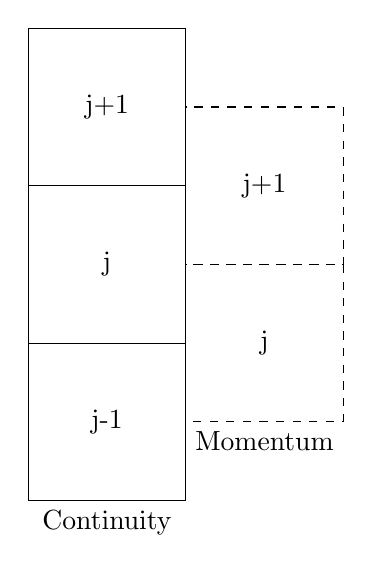
\begin{tikzpicture}
\draw (-2,-3) rectangle +(2,2);
\node[anchor=center] at (-1,-2) {j-1};
\draw (-2,-1) rectangle +(2,2);
\node[anchor=center] at (-1, 0) {j};
\draw (-2, 1) rectangle +(2,2);
\node[anchor=center] at (-1, 2) {j+1};
\draw[dashed] (-0,-2) rectangle +(2,2);
\node[anchor=center] at (1, -1) {j};
\draw[dashed] (-0, 0) rectangle +(2,2);
\node[anchor=center] at (1, 1) {j+1};
\node[anchor=north] at (-1, -3) {Continuity};
\node[anchor=north] at (1, -2) {Momentum};
\end{tikzpicture}
\caption{Illustration of indexing scheme.}
\label{fig:vertical_pipe_with_cells}
\end{figure}

Recalling the staggered mesh from \sect{sect:geometry}, the six scalar conservation laws, \eqref{eqn:conservation_of_ncg} -- \eqref{eqn:con_energy_liq}, are each integrated over the continuity volumes.
The assumption in these integrals is that the value of the conserved quantities and all thermodynamically-related variables are constant within a given volume.
\fig{fig:constant_value} shows a graphical representation of this idea for a generic function $f(x)$ over several spatial continuity volumes. 

\begin{figure}[ht]
\centering
\tikzsetnextfilename{images/constant_value_pdf}
\begin{tikzpicture}
\draw [->, thick] (-5,0) -- (6,0);
\draw [->, thick] (-5,0) -- (-5,4);
\draw (-4,1) -- (-1,1);
\draw (-1,2) -- (2,2);
\draw (2,3) -- (5,3);
\draw (-5.5,3) node {$f(x)$};
\draw [dashed] (-4,1) -- (-4,0);
\draw [dashed] (-1,2) -- (-1,0);
\draw [dashed] (2,3) -- (2,0);
\draw [dashed] (5,3) -- (5,0);
\foreach \x / \xtext in {-2.5/x_{j-1},-1/x_{j-\onehalf},0.5/x_j,2/x_{j+\onehalf},3.5/x_{j+1}}
	\draw [thick] (\x,-2pt) -- (\x,0pt) node [anchor=north] {$\xtext$};
\end{tikzpicture}
\caption{Constant variable values within computational volumes.}
\label{fig:constant_value}
\end{figure}

Within a channel, a given continuity volume has a constant cross-sectional area, $A_{c_{j}}$, and a length of $\Delta x_{j}$.
The cross-sectional area of the boundary between two continuity volumes is given by the cross-section area of the momentum volume at that boundary, $A_{m}$.
The volume integrated equation is given by \eqref{eqn:spatially_discrete_liq_m_con}.
For illustrative purposes, \eqref{eqn:conservation_of_liq} will be integrated over a given volume, $V_j$, as shown in \fig{fig:single_volume}.

\begin{figure}[h!t]
\centering
\begin{tikzpicture}
\draw [thick] (-2,-3) rectangle (2,3);
\draw [<->] (3.5,-3) -- (3.5,3);
\draw (3.25,-3) -- (3.75,-3);
\draw (3.25,3) -- (3.75,3);
\draw (4,0) node {$\Delta x_j$};
\draw [<->] (-2,-3.75) -- (2,-3.75);
\draw (-2,-3.5) -- (-2,-4);
\draw (2,-3.5) -- (2,-4);
\draw (0,-4.25) node {$A_{C,j}$};
\draw [dashed] (-2,0) -- (2,0);
\filldraw [black] (0,0) circle (2pt);
\foreach \y/\ytext in {-3/$x_{j-\onehalf}$,0/$x_j$,3/$x_{j+\onehalf}$}
	\draw (2,\y) node [anchor=west] {\ytext};
\end{tikzpicture}
\caption{Single volume over which the conservation equations are integrated.}
\label{fig:single_volume}
\end{figure}

For the mass-flux terms evaluated on the continuity volume edge, the advected quantity is evaluated using a 1st order upwind method \cite{Tannehill1997}.
The velocity and cross-sectional area utilized in the continuity flux terms, $u_j$ and $A_{m,j}$, have the values defined in the momentum volume that aligns with the boundary of continuity volumes.
The sign of the velocity at the volume boundary determines the value of the donored quantity, $\ave{a}_{d,j \pm \onehalf}$.
A generic formulation for this scheme is given by \eqref{eqn:upwind_donoring}.
The same general procedure is used for the other five scalar conservation equations.

\begin{IEEEeqnarray}{lcl}
\int_{V_j}\frac{\partial \left(\alpha_l \rho_l \right)}{\partial t } & + & \nabla \cdot \left( \alpha_l \rho_l u_l \right) \mathrm{d}V = \int_{V_j} \left(-(1-\eta)\Gamma^{'''} - S^{'''} + s_{m,l}\right) \mathrm{d}V \nonumber \\
V_j \frac{\partial \left(\alpha_{l,j} \rho_{l,j} \right)}{\partial t } & = & -\int_{V_j}\nabla \cdot \left( \alpha_l \rho_l u_l \right) \mathrm{d}V -(1-\eta_j)\Gamma_j - S_j + s_{m,l,j}V_j \nonumber \\
V_j \frac{\partial \left(\alpha_{l,j} \rho_{l,j} \right)}{\partial t } & = & -\left[\alpha_l \rho_l u_l A_{m}\right]_{x_{j-\onehalf}}^{x_{j+\onehalf}} -(1-\eta_j)\Gamma_j - S_j + s_{m,l,j}V_j \nonumber \\
\label{eqn:spatially_discrete_liq_m_con}
V_j \frac{\partial \left(\alpha_{l,j} \rho_{l,j} \right)}{\partial t } & = & -\left( \don{\alpha_l \rho_l}_{d,j+\onehalf} u_{l,j+1} A_{m,j+1} - \don{\alpha_l \rho_l}_{d,j-\onehalf} u_{l,j} A_{m,j}\right) \nonumber \\
& & -(1-\eta)\Gamma_j - S_j + s_{m,l,j}V_j
\end{IEEEeqnarray}

\begin{equation}
\label{eqn:upwind_donoring}
\ave{a}_{d, j - \onehalf} = \begin{cases} a_{j-1} &  u_j \geq 0 \\ a_{j} & u_j < 0 \end{cases}
\end{equation}

The three momentum conservation equations, \eqref{eqn:con_mom_liq} -- \eqref{eqn:con_mom_ent}, are integrated over their momentum volume.
The cross-sectional area for a momentum volume, $A_{m,j}$, can be defined independently of the two cross-sectional areas of the adjoining continuity volumes.
The momentum flux terms, \eqref{eqn:momentum_flux_terms}, are treated similarly to the flux terms in the continuity equations.

\begin{equation}
\label{eqn:momentum_flux_terms}
-\left[<\alpha_l \rho_l u_l>_{d} u_l \tilde{A}\right]_{x_{j-\onehalf}}^{x_{j + \onehalf}}
\end{equation}

There are two primary differences.
First, the area in the flux term, $\tilde{A}$, is taken as the minimum of two areas from the adjoining momentum volumes, \eqref{eqn:area_def}.

\begin{equation}
\label{eqn:area_def}
\min\left(A_{m,j}, A_{m,j+1}\right)
\end{equation}

Second, the velocity that is used to determine the origin of the donored quantity is the arithmetic mean of the velocities from the two adjacent momentum volumes, \eqref{eqn:average_advecting_vel}.

\begin{equation}
\label{eqn:average_advecting_vel}
u_{k,j+\frac{1}{2}} = \frac{1}{2}\left(u_{k,j} + u_{k, j+1}\right)
\end{equation}

The ordering of the governing equations within a given continuity volumes is as follows:

\begin{enumerate}
\item{Conservation of the \ncg{} field mass.}
\item{Conservation of the vapor field mass.}
\item{Conservation of the gaseous phase energy.}
\item{Conservation of the liquid phase energy.}
\item{Conservation of the entrained liquid field mass.}
\item{Conservation of the continuous liquid field mass.}
\end{enumerate}

The conservation of momentum equations within a given momentum volume are ordered as follows:

\begin{enumerate}
\item{Conservation of the continuous liquid field momentum.}
\item{Conservation of the gaseous phase momentum.}
\item{Conservation of the entrained liquid field momentum.}
\end{enumerate}

%-------------------------------------------------------------------------------
%-------------------------------------------------------------------------------
%-------------------------------------------------------------------------------
\subsection{Temporal Approximations}
\label{subsect:temporal_approx}

Once the governing conservation equations have been spatially discretized utilizing the method outlined above, the temporal derivatives need to be approximated numerically.
The continuous conservation equations, \eqref{eqn:conservation_equations}, are now a spatially-discrete, temporally-continuous set of equations given by \eqref{eqn:temporal_semi_discrete}, where $\vec{E}$ now represents the spatially discrete approximation of $\vec{e}$.

\begin{equation}
\label{eqn:temporal_semi_discrete}
\frac{\partial \,\vec{y} }{\partial t} = \vec{E}(\vec{y}(t))
\end{equation}

Given that there are nine conservation equations, nine independent parameters need to be chosen.
The choice of the nine variables that will be solved for is another distinguishing characteristic of safety analysis software.
\cobra{} uses the following set of nine independent variables \eqref{eqn:independent_variables}.

\begin{equation}
\label{eqn:independent_variables}
\vec{x} = [\alpha_{g}P_{n}, \alpha_g, \alpha_g h_v, (1 - \alpha_g) h_l, \alpha_e, P, \dot{m}_g, \dot{m}_l, \dot{m}_e]^{T}
\end{equation}

The definition of $\dot{m}_k$ is given by \eqref{eqn:mom_dot}.

\begin{equation}
\label{eqn:mom_dot}
\dot{m}_{k} = \ave{\alpha_k \rho_k}_{a} u_{k} A_{m}
\end{equation}

The averaging operator $\ave{a}_{a}$ provides the average of a quantity from the two adjoining continuity volumes, \eqref{eqn:average_val}.

\begin{equation}
\label{eqn:average_val}
\ave{a}_{a,j} = \frac{a_{j} + a_{j+1}}{2}
\end{equation}

The choice of independent parameters used in \cobra{} is not the only option.
Other software, such as TRACE and RELAP5-3D, use variants of these parameters.
These variations include the use of velocities instead of momenta and temperatures or internal energies instead of enthalpies \cite{RELAP, TRACE}.

A distinguishing feature of the numerical method in \cobra{} is its treatment of the temporal derivative for the conservation of momentum.
In the work that follows the temporal derivative of the conserved momentum equations is directly discretized, which is known as the conservative form.
The other option, the non-conservative form, is to expand analytically the temporal derivative via the chain rule, \eqref{eqn:non_conservative}, and these equations are then temporally discretized.

\begin{equation}
\label{eqn:non_conservative}
\frac{\partial \alpha_k \rho_k u_k}{\partial t} = \alpha_k \rho_k \frac{\partial u_k}{\partial t} + u_k \frac{\partial \alpha_k \rho_k}{\partial t}
\end{equation}

Within \cobra{} the temporal derivative is approximated by a one-step difference scheme, \eqref{eqn:simple_partial_t}, where the continuous time variables are now evaluated at discrete points, $t^0, t^1, \ldots, t^N$.
The notations $t^0$ and $t^N$ represent the initial and final time, respectively.
The term ''one-step" refers to the fact that the temporal derivative involves only two consecutive points in time.

\begin{IEEEeqnarray}{rcl}
\int^{t^{n+1}}_{t^n}\frac{\partial \vec{y}(\vec{x})}{\partial t}\mathrm{d}\tau & = & \int^{t^{n+1}}_{t^n}\vec{E}(\vec{y}(\vec{x}))\mathrm{d}\tau \nonumber \\
\vec{y}(\vec{x}^{n+1}) - \vec{y}(\vec{x}^{n}) & = & \int_{t^{n+1}}^{t^n}\vec{E}(\vec{y}(\vec{x}))\mathrm{d}\tau \nonumber  \\
\vec{y}(\vec{x}^{n+1}) - \vec{y}(\vec{x}^{n}) & = & \Delta t \vec{E}(\vec{y}(\vec{x}^{*})) \nonumber  \\
\label{eqn:simple_partial_t}
\frac{\vec{y}(\vec{x}^{n+1}) - \vec{y}(\vec{x}^{n})}{\Delta t} & = & \vec{E}(\vec{y}(\vec{x}^{*}))
\end{IEEEeqnarray}

The choice of how to approximate the temporal integral of the sources and sinks of the system, $\vec{E}(\vec{y}(\vec{x}^{*}))$, hereafter referred to as $\vec{E}^{*}$, is a factor that defines the eventual solution algorithm.
There are two subcategories for solving this one-step temporal-integration problem, single-stage and multi-stage \cite{Stewart1981,LeVeque2007}.
\alg{alg:single_stage_temporal} shows how a multi-stage temporal integration scheme would work.

\begin{algo}[H]
\setlength{\baselineskip}{0.625\baselineskip}
\begin{algorithmic}[1]
\Require $\vec{y}^{0}$ and $t^{0}$
\Set $n = 0$
\Loop \; Transient Loop
    \State $t^{n+1} : = t^{n} + \Delta t$
    \For{$j = 1 \to J$} \; Stage Loop
		\BlackBox Solve $\displaystyle \frac{\vec{y}^{j} - \vec{y}^{n}}{\Delta t} =  \vec{E}_{j}^{*}$ for $\vec{y}^{j}$.
	\EndFor
	\State $n = n + 1$
\EndLoop
\end{algorithmic}
\caption{Multi-stage temporal integration scheme.}
\label{alg:single_stage_temporal}
\end{algo}

The final-stage conserved variables will be the new-time variables, $\vec{y}^{J} = \vec{y}^{n+1}$. 
At each stage the choice of how to approximate the driving function, $\vec{E}_{j}^{*}$, can change in both its functional dependence upon the stage values of $\vec{y}^{j}$ and in which components of $\vec{E}^{*}$ are included.
By excluding certain portions of $\vec{E}^{*}$ at certain stages, a time-splitting algorithm is developed.
Time-splitting algorithms are also known as operator-splitting algorithms. 
By changing the functional dependencies of terms within $\vec{E}^{*}$ at different stages, predictor-corrector methods, also called stabilizing correction methods, are generated. 
A single-stage method is the degenerate multi-stage case of $J = 1$.

The conserved quantities within a continuity volume are nonlinear functions of the chosen independent parameters, \eqref{eqn:nonlinear_functions}, regardless of the approximation chosen for $\vec{E}^{*}$.

\begin{equation}
\label{eqn:nonlinear_functions}
\vec{y}^{n+1} = \vec{y}(\vec{x}^{n+1})
\end{equation}

This nonlinearity necessitates the use of a nonlinear solver at every timestep.
Any dependence of $\vec{E}^{*}$ on the new-time parameters can create additional nonlinearities.
The semi-discrete formulation, \eqref{eqn:simple_partial_t}, is expressed as a fully-discrete nonlinear function of $\vec{x}$ by \eqref{eqn:nonlinear_residuals}.

\begin{equation}
\label{eqn:nonlinear_residuals}
\vec{F}(\vec{x}^{n+1}) = \vec{y}(\vec{x}^{n+1}) - \vec{y}(\vec{x}^n) -\Delta t \vec{E}^{*}
\end{equation}

Depending upon the approximation of $\vec{E}^{*}$ and the number of stages, the temporal integration method used has an associated temporal accuracy.
The temporal accuracy is a way of quantifying the behavior of the solution as the timestep is reduced.
Order of accuracy estimates for temporal integration techniques are proportionality statements between the numerical error and a power of the timestep, $\mathcal{O}(\Delta t^k)$ \cite{LeVeque2007}. 
However, it has been shown that if the nonlinear problem, \eqref{eqn:nonlinear_residuals}, is not solved at every time step, the temporal accuracy of a method can be degraded \cite{Knoll2001, Mahaffy1993}.

%-------------------------------------------------------------------------------
%-------------------------------------------------------------------------------
%-------------------------------------------------------------------------------
\subsection{Nonlinear Approximations}
\label{subsect:nonlinear_approximations}

The method used to solve \eqref{eqn:nonlinear_residuals} for $\vec{x}^{n+1}$ in this work is Newton's method \cite{Deuflhard2004, Dennis1996}.
The nonlinear residual being solved is a function of the new-time unknowns, $\vec{x}^{n+1}$.
Newton's method is an iterative procedure to obtain $\vec{x}^{*}$ such that $\vec{F}(\vec{x}^{*}) = 0$.
Since Newton's method is an iterative procedure for obtaining the correct new-time variables, two superscripts are required.
The nonlinear iterate superscript will be $k$.
Successive linearization of the nonlinear problem \eqref{eqn:newton_taylor} generates an iterative solution method.

\begin{IEEEeqnarray}{rcccl}
0 & = & \vec{F}(\vec{x}^{n+1,k}+\vec{\delta x}^k) & = & \vec{F}(\vec{x}^{n+1,k}) +  \int_{\vec{x}^{n+1,k}}^{\vec{x}^{n+1,k}+\vec{\delta x}^k}\frac{\partial \vec{F}}{\partial \vec{x}}(\vec{z}) \mathrm{d} \vec{z} \nonumber \\
\label{eqn:newton_taylor}
0 & = & \vec{F}(\vec{x}^{n+1,k}+\vec{\delta x}^k) & \approx & \vec{F}(\vec{x}^{n+1,k}) + \vec{J}(\vec{x}^{n+1,k}) \cdot \vec{\delta x}^k
\end{IEEEeqnarray}

The algorithm is then one of finding successive updates, $\vec{\delta x}^k = \vec{x}^{n+1,k+1} - \vec{x}^{n+1,k}$, by solving \eqref{eqn:newton}.

\begin{equation}
\label{eqn:newton}
\vec{J}(\vec{x}^{n+1,k})\cdot \vec{\delta x}^k = -\vec{F}(\vec{x^{n+1,k}})
\end{equation} 

Since the system of nonlinear equations being solved represents a transient simulation, the iterations at each timestep start with an initial guess for the new-time variables that is equal to the old-time variables, $\vec{x}^{n+1,0} = \vec{x}^{n}$.
The underlying assumption of this initial value is that the independent parameters will not change greatly over a timestep, and the old-time variables will provide an initial vector that is within the radius of convergence of Newton's method.
\alg{alg:local_newton} provides an overview of a transient simulation using a Newton's method for a single-stage temporal integration scheme.
The algorithm generalizes to a multi-stage temporal integration method by enclosing the Newton loop within a stage loop.

\begin{algo}[H]
\setlength{\baselineskip}{0.625\baselineskip}
\begin{algorithmic}[1]
\Require $\vec{x}^{0}$ and $t^{0}$
\Set $n = 0$
\Loop \; Transient Loop
    \State $t^{n+1} : = t^{n} + \Delta t$
    \State $k = 0$
    \State $\vec{x}^{n+1,k} = \vec{x}^{n}$
    \Loop \; Newton Loop
		\Calculate $\vec{F}(\vec{x}^{n+1,k})$ and $\vec{J}(\vec{x}^{n+1,k})$
		\Calculate $\vec{\delta x}^k = - \vec{J}^{-1}\cdot\vec{F}$
		\BlackBox $\vec{x}^{n+1,k+1}$
		\State $k = k + 1$
		\BlackBox Loop Termination Criteria
	\EndLoop
	\State $n = n + 1$
\EndLoop
\end{algorithmic}
\caption{Local Newton's method for single-stage temporal integration.}
\label{alg:local_newton}
\end{algo}

In \alg{alg:local_newton}, there are two black box calculations: the calculation of the updated independent parameters, $\vec{x}^{n+1,k+1}$, and the calculation of the loop termination criteria.
In the case of the loop termination criteria being $k > 0$ the resultant method is labeled as a single-shot linearization.
The exact nature of those two black box calculations is method-dependent and various options will be discussed later.
In multi-stage temporal integration methods both the update method and the loop termination criteria may vary between stages. 

%-------------------------------------------------------------------------------
%-------------------------------------------------------------------------------
%-------------------------------------------------------------------------------
\section{Solution Methods}
\label{sect:solution_techniques}

\sect{sect:numeric_approximation} provided a framework for characterizing the different methods used in thermal-hydraulic safety codes. 
Each method can be defined by the manner in which the temporal integration is carried out and the manner in which the nonlinearities are resolved.
The methods described below form the core of available techniques that have been developed for two-phase safety analysis codes. 
While each of the following methods may have many subtly varying algorithmic implementations that have appeared in safety analysis software, the algorithms detailed below are general enough to encompass these variants.

%-------------------------------------------------------------------------------
%-------------------------------------------------------------------------------
%-------------------------------------------------------------------------------
\subsection{Fully Explicit Method}
\label{subsect:numerics_explicit}
The least computationally expensive method on a per timestep basis for temporally integrating \eqref{eqn:simple_partial_t} is a single-stage, fully explicit method.
In the fully explicit method, the driving function is approximated as $\vec{E}(\vec{x}^n)$.
The nonlinear vector notation formulation for this method is given by \eqref{eqn:explicit}.

\begin{equation}
\label{eqn:explicit}
\vec{F}(\vec{x}^{n+1}) = \vec{y}(\vec{x}^{n+1}) - \vec{y}^{n} - \Delta t \vec{E}(\vec{y}(\vec{x}^{n}))
\end{equation}

The algorithmic implementation is shown in \alg{algo:explicit}.
Given the choice of independent parameters in \cobra{}, there are nonlinearities present in the temporal derivative.
While the momentum conservation equations have the identity matrix, $\vec{I}$, for their temporal Jacobian, the continuity equations' temporal Jacobian is a [6x6] matrix with no inter-volume coupling terms.

\begin{algo}[H]
\setlength{\baselineskip}{0.625\baselineskip}
\begin{algorithmic}[1]
\Require $\vec{x}^{0}$ and $t^{0}$
\Set $n = 0$
\Loop \; Take a Time Step
    \State $t^{n+1} : = t^{n} + \Delta t$
    \Calculate $\vec{F}(\vec{x}^n)$ and $\vec{J}(\vec{x}^n)$
    \Calculate $\vec{\delta x} = -\vec{J}^{-1}\vec{F}$
    \Calculate $\vec{x}^{n+1} = \vec{x}^{n} + \vec{\delta x}$ 
\EndLoop{\;$n = n+1$}
\end{algorithmic}
\caption{Single-stage, fully explicit, single-shot linearization method.}
\label{algo:explicit}
\end{algo}

While this particular method is the least computationally expensive on a per timestep basis, it has a severe weakness.
That weakness is the Courant-Friedrichs-Lewy (CFL) limit imposed upon the time step size, $\Delta t$.
The CFL limit is a relationship between the spatial and temporal discretization and the characteristic velocities of information propagation in the problem of interest \cite{LeVeque2007, Tannehill1997}.
For the case of \eqref{eqn:explicit}, the CFL limit is given in \eqref{eqn:cfl_explicit}.

\begin{equation}
\label{eqn:cfl_explicit}
\Delta t_j \lesssim \frac{\Delta x_j}{|u_j|+|c_j|}
\end{equation}

In \eqref{eqn:cfl_explicit}, $c_j$ and $u_j$ are the speed of sound and the magnitude of a given phasic velocity, respectively, at a given location within the domain.
Using the local fluid conditions, $\Delta t_j$ is calculated at every point within the domain.
The $\Delta t$ chosen for the $t^{n} \rightarrow t^{n+1}$ timestep is the most restrictive calculated value over the domain.
While the explicit method may provide the lowest computational cost on a per-timestep basis, the number of timesteps required for a given problem will be much greater due to this restrictive CFL limitation.

\begin{equation}
\label{eqn:global_cfl}
\Delta t = \min_{j \in \Omega} \Delta t_j
\end{equation}

Put another way, the maximum permissible timestep size is determined by the most restrictive CFL limit within the domain.
Since the CFL limit is based upon the local speed of sound it is referred to as the sonic Courant limit.
This limitation of the explicit method prompted the development of alternative methods that were capable of exceeding this Courant limit.

%-------------------------------------------------------------------------------
%-------------------------------------------------------------------------------
%-------------------------------------------------------------------------------
\subsection{Fully Implicit Method}
\label{subsect:numerics_fully_implicit}
One alternative method for integrating \eqref{eqn:temporal_semi_discrete} is to use a fully implicit discretization of $\vec{E}^{*}$ \cite{Frepoli2003, Barre1990}.
The fully implicit method temporally approximates $\vec{E}^{*}$ as a function  of new-time parameters only, \eqref{eqn:implicit}.

\begin{equation}
\label{eqn:implicit}
\vec{F}(\vec{x}^{n+1}) = \vec{y}(\vec{x}^{n+1}) - \vec{y}^{n} - \Delta t \vec{E}(\vec{y}(\vec{x}^{n+1}))
\end{equation}

This method has the advantage of not being limited by a CFL number.
While this allows for greatly increased timesteps to be taken, the numerical scheme introduces nonphysical diffusion into the solution \cite{Mahaffy1993}.
Additionally, the solution of \eqref{eqn:implicit} is the most computationally expensive on a per timestep basis of the methods considered.
This computational expense comes from the full inter-volume coupling of the Jacobian matrix during the nonlinear solve.
The computational implementation of a fully implicit method is presented in \alg{algo:implicit}.

\begin{algo}[H]
\setlength{\baselineskip}{0.625\baselineskip}
\begin{algorithmic}[1]
\Require $\vec{x}^{0}$ and $t^{0}$
\Set $n = 0$
\Loop \; Transient Loop
    \State $t^{n+1} : = t^{n} + \Delta t$
    \For{$j = 1 \to 2$} \; Stage Loop
    \State $k = 0$
    \State $\vec{x}^{k} = \vec{x}^{n}$
    \Loop \; Newton Loop
		\Calculate $\vec{F}(\vec{x}^{k})$ and $\vec{J}(\vec{x}^{k})$
		\Calculate $\vec{\delta x}^k = - \vec{J}^{-1}\cdot\vec{F}$
		\BlackBox $\vec{x}^{k+1}$
		\State $k = k + 1$
		\BlackBox Loop Termination Criteria
	\EndLoop	
	\EndFor
	\State $n = n + 1$
\EndLoop
\end{algorithmic}
\caption{Fully implicit, two-stage, nonlinear-solver method.}
\label{algo:implicit}
\end{algo}

%-------------------------------------------------------------------------------
%-------------------------------------------------------------------------------
%-------------------------------------------------------------------------------
\subsection{Semi-Implicit Method}
\label{subsect:semi_implicit}

Another alternative method for integrating \eqref{eqn:temporal_semi_discrete} is the semi-implicit method.
It was developed to overcome the sonic Courant limitations of the explicit method while avoiding both the high computational cost and excessive diffusivity of the fully implicit method \cite{Liles1978}.
There are two distinguishing characteristics of the semi-implicit method: the pressure gradient terms in the momentum conservation equations and the velocities for the advection of mass and energy use new-time variables. 
The implicit evaluation of the pressure gradient in the momentum equations is what leads to a CFL limit known as the material Courant limit.
Similar to the sonic Courant limit discussed in \sect{subsect:numerics_explicit}, the material Courant limit dictates the largest $\Delta t$ that can be achieved while maintaining a stable solution algorithm.
In this method the Courant limit is given by \eqref{eqn:si_cfl}.

\begin{equation}
\label{eqn:si_cfl}
\Delta t_j \lesssim \frac{\Delta x_j}{|u_{k,j}|}
\end{equation}

The characteristic velocity used in the calculation of the Courant limit is based on the phasic velocity only.
This allows for larger, but still limited, timestep sizes than the explicit method.
The limit on timestep size is due to the explicit evaluation of the donored quantities in the flux terms in the conservation equations.
As stated, the flux of mass and energy include new-time velocities, $u^{n+1}_k$.
Since \cobra{} uses momenta, $\dot{m}_{k}$, as independent parameters, the velocities are derived quantities, whose functional form is given in \eqref{eqn:si_vel}.
The $\ave{\alpha_k \rho_k}^{n}_{a}$ represents the arithmetic average of macroscopic densities from adjoining continuity volumes.

\begin{equation}
\label{eqn:si_vel}
u^{n+1}_{k, j \pm \onehalf} = \frac{\dot{m}^{n+1}_{k, j \pm \onehalf}}{A_{m, j \pm \onehalf} \ave{\alpha_{k} \rho_{k}}^{n}_{a, j \pm \onehalf}} 
\end{equation}

The donoring operator $\don{a}^{n}_{d}$ is an extension of \eqref{eqn:upwind_donoring}.
The donored quantities and the velocities used to determine the direction of donoring are evaluated with their old-time values.

\alg{alg:si_legacy} shows the algorithm for solving the semi-implicit method.

\begin{algo}[H]
\setlength{\baselineskip}{0.625\baselineskip}
\begin{algorithmic}[1]
\Require $\vec{x}^{0}$ and $t^{0}$
\Set $n = 0$
\Loop \; Transient Loop
    \State $t^{n+1} : = t^{n} + \Delta t$
	\Calculate $\vec{F}(\vec{x}^{n})$ and $\vec{J}(\vec{x}^{n})$
	\BlackBox $\vec{\delta x} = - \vec{J}^{-1}\cdot\vec{F}$
	\Calculate $\vec{x}^{n+1} = \vec{x}^{n} + \vec{\delta x}$
	\State $n = n + 1$
\EndLoop
\end{algorithmic}
\caption{\cobra{} Semi-Implicit method.}
\label{alg:si_legacy}
\end{algo}

%-------------------------------------------------------------------------------
%-------------------------------------------------------------------------------
%-------------------------------------------------------------------------------
\subsection{Stability-Enhancing Two-Step Method} 
\label{subsect:numerics_sets}
In order to overcome the material Courant limit placed upon simulations by the semi-implicit method, the Stability Enhancing Two-Step (SETS) method was developed \cite{Mahaffy1982}.
While not as stable as the fully implicit method, the SETS method allows for timesteps to exceed the material Courant limit.
It overcomes the material Courant limit by taking a multi-stage approach to the temporal integration.
While there are variants of the SETS method \cite{TRACE}, \alg{alg:sets} reflects the original publication.
The outline below uses velocities as independent parameters, not momenta.

There are three stages in the original SETS method.
Stage one is a single-shot linearized solution of the momentum equations where only the velocity terms in the momentum equations of $\vec{E}^{*}$ are evaluated implicitly.
This first stage only involves the solution of the momentum equations; the mass and energy equations are not solved during this step.
The lack of implicit dependence upon any continuity variables allows for coupling only between momentum volumes.
This step results in predicted $u^{*}_{k}$ phasic velocities.

In stage two, the momentum and continuity equations are solved using a traditional semi-implicit scheme with two exceptions.
The first is that the momentum flux terms are evaluated using the stage-one predicted velocities as the advecting velocities instead of explicitly evaluating them.
The second is that the nonlinearities in the momentum equations, arising from interfacial and wall drag, are subject to a single-shot linearization.
The single-shot nature of the momentum equations allows for the reduction of the system into coupled continuity volumes as in the semi-implicit method.
The nonlinear continuity equations are then solved via Newton's method.
Stated another way, the Jacobians for the momentum equations are fixed at their first Newton iterate value, while the Jacobians for the mass and energy equations are updated at each iterate.

In the third stage the mass and energy equations are solved such that all continuity variables are implicitly evaluated and the velocities are from stage two.
The only results from stage two that are used in stage three are the velocities, $\vec{u}^{n+1}$.
The resulting system of coupled continuity equations is then solved.
This final stage allows timestep sizes that exceed the material Courant limit.
For each stage the residual and Jacobian matrix will be denoted by $\vec{F}_k$ and $\vec{J}_k$, with $k = 1 \to 3$.

\begin{algo}[H]
\setlength{\baselineskip}{0.625\baselineskip}
\begin{algorithmic}[1]
\Require $\vec{x}^{0}$ and $t^{0}$
\Set $n = 0$
\Loop \; Transient Loop
    \State $t^{n+1} : = t^{n} + \Delta t$
	\Calculate $\vec{F}_1$ and $\vec{J}_1$
	\Calculate $\vec{u}^{*}$ from $\vec{\delta u}^{*} = -\vec{J}^{-1}_1\vec{F}_1$
	\Loop \; Newton Loop
		\Calculate $\vec{F}_2$ and $\vec{J}_2$
		\BlackBox $\vec{\delta x} = - \vec{J}_2^{-1}\vec{F}_2$
		\Calculate $\vec{x}^{n+1} = \vec{x}^{n} + \vec{\delta x}$
		\BlackBox Loop Termination Criteria
	\EndLoop
	\Calculate $\vec{x}^{n+1}$ from $\vec{F}_3$.
	\State $n = n + 1$
\EndLoop
\end{algorithmic}
\caption{SETS method.}
\label{alg:sets}
\end{algo}

This algorithm was designed to allow existing software utilizing the semi-implicit method to be embedded within a larger framework.
The loop termination criteria is an implementation-specific choice.
The TRACE code uses an $L_{\infty}$ norm of the unscaled Newton updates for the continuity variables to determine convergence.

%-------------------------------------------------------------------------------
%-------------------------------------------------------------------------------
%-------------------------------------------------------------------------------
\subsection{Nearly-Implicit Method}
\label{subsect:numerics_nearly_implicit}
Another possible method used to overcome the material Courant limit without incurring the same computational cost as the fully implicit method is the Nearly-Implicit method \cite{Trapp1986, RELAP}.
The Nearly-Implicit method is a multi-stage temporal integration scheme.
In the first stage the approximation  of $\vec{E}^{*}$ is one in which the mass and energy terms are implicit except for the donored values in the flux terms. 
In addition, the the chain rule is applied to the continuous temporal derivatives, resulting in mass equations similar to \eqref{eqn:ni_dt}.
The energy temporal derivatives are similarly expanded.

\begin{equation}
\label{eqn:ni_dt}
\frac{\partial \alpha_k \rho_k}{\partial t} = \alpha_k \frac{\partial \rho_k}{\partial t} + \rho_k \frac{\partial \alpha_k}{\partial t}
\end{equation}

The temporal discretization of \eqref{eqn:ni_dt} is given by \eqref{eqn:ni_dis_dt}.

\begin{equation}
\label{eqn:ni_dis_dt}
\alpha_k \frac{\partial \rho_k}{\partial t} + \rho_k \frac{\partial \alpha_k}{\partial t} = \alpha^n_k\frac{ \rho^{n+1}_k - \rho^{n}_k}{\Delta t} + \rho^{n}_k\frac{\alpha^{n+1}_k - \alpha^{n}_k}{\Delta t}
\end{equation}

The momentum equations are implicit in their momentum flux, pressure, and interfacial exchange terms.

The Nearly-Implicit method is a three-stage solution process.
The first stage is similar to the semi-implicit method.
However, as opposed to the semi-implicit method where the momentum variables are eliminated from the equations being solved, the Nearly-Implicit method uses the mass and energy equations to eliminate the pressure terms from the momentum equations.
The resulting matrix is a linear system of coupled velocities.
The stage-one velocities are taken to be the new-time velocities.
Once the stage-one velocities are obtained, the corresponding stage-one continuity variables are obtained analogously to the new-time momentum in the semi-implicit method.
Stage one is a single-shot linearization.
In the second stage, only the continuity equations are solved and they are in conservative form.
The interfacial exchange terms in the mass and energy equations are evaluated using the stage-one continuity variables.
The resulting system of equations is linear in the conserved quantities.
This linear system is solved for the conserved quantities.
In stage three, the nonlinear relation between the conserved quantities and the independent parameters is then approximated via a single-shot linearization of the equations of state.
\alg{alg:ni} shows the three-stage process.

\begin{algo}[H]
\setlength{\baselineskip}{0.625\baselineskip}
\begin{algorithmic}[1]
\Require $\vec{x}^{0}$ and $t^{0}$
\Set $n = 0$
\Loop \; Transient Loop
    \State $t^{n+1} : = t^{n} + \Delta t$
	\Calculate $\vec{F}_1$ and $\vec{J}_1$
	\Calculate $\vec{c}^{*}$ and $\vec{u}^{n+1}$ from $\vec{\delta x}^{*} = -\vec{J}^{-1}_1\vec{F}_1$
	\Calculate $\vec{F}_2$
	\Calculate $\vec{c}^{**}$ from $\vec{F}_2$
	\Calculate $\vec{c}^{n+1}$ from $\vec{F}_3$.
	\State $n = n + 1$
\EndLoop
\end{algorithmic}
\caption{Nearly-Implicit method}
\label{alg:ni}
\end{algo}

%-------------------------------------------------------------------------------
%-------------------------------------------------------------------------------
%-------------------------------------------------------------------------------
\section{Domain Coupling}
\label{sect:code_coupling}

\cobra{} possesses models of the physics necessary to simulate the complicated in-core flow patterns and heat transfer encountered during a postulated LOCA.
However, it lacks the detailed models for NPP components (pumps, valves, accumulators, pressurizers) that are traditionally available from system analysis codes.
When modeling full NPP transients, it is advantageous to use sub-channel software for the core and system analysis software for the rest of the NPP.
The combination of different specialized software is a common practice.
This coupling of capabilities can be accomplished in two ways: the two pieces of software can be merged or they can be coupled via data exchange.
Examples of the first method are MARS \cite{Jeong2008}, COBRA/TRAC \cite{Thurgood1983c}, and TRACE \cite{TRACE}.
Coupling software via data exchange is a more common option \cite{Makihara2003, Aumiller2002, Aumiller2001, Avramova2006, Weaver2002, Rodriguez2002}, and it will be discussed below.

When coupling via data exchange, the use of explicit coupling can lead to a sonic Courant limit imposed at the boundary of the two coupled systems \cite{Ragusa2009, Aumiller2001}.
To circumvent the sonic Courant limit, a semi-implicit method for the coupling of software via data exchange has been developed for thermal-hydraulic simulations \cite{Weaver2002, Aumiller2002}.
This coupling technique allows for the material Courant limit to be uniformly applied across the two pieces of software.
This technique is of direct interest to the proposed research.

The coupling of the different software involves the use of a third-party message passing interface.
The program used for the software coupling in the papers of interest is the Parallel Virtual Machine (PVM) \cite{Geist1994}.
PVM allows the data exchange to occur between the coupled software.
As originally formulated, the software coupling technique involves decomposing the coupled problem into two pieces, the master and the slave domains.
In this respect, the problem can be thought of as being decomposed into a subdomain controlled by a master program and a slave domain being controlled by a slave program.
The presentation of the method is in terms of the RELAP5-3D conservation equations, which are different from those in \cobra{}.
The coupling method first developed presented RELAP5-3D as both the master and slave software \cite{Weaver2002}.
Later work showed how this base method could be extended to allow coupling between RELAP5-3D and the \cobra{} subchannel analysis software \cite{Aumiller2002}.
This reformulation was designed to allow for a consistent transition between a two-phase, two-field based solver and and a two-phase, three-field based solver. 
A short outline of the method as formulated for RELAP5-3D coupling is presented below.

The semi-implicit domain decomposition is accomplished via the staggered mesh formulation.
The master domain is truncated on a continuity volume.
The fluxes of conserved continuity quantities at the boundary of the coupled volumes are retained as unknowns during the formulation of the global pressure matrix.
Upon forming the pressure matrix, the Newton update for the pressures will be expressed as a linear combination of all of the unknown mass and energy fluxes through the coupled boundaries of the domain, \eqref{eqn:si_relap} \cite{Weaver2002}.

\begin{IEEEeqnarray}{rcl}
\label{eqn:si_relap}
\delta P^{n+1}_{k} = a_k & + & 
\sum_{j = 1}^{N_c} b_{k,j}n_{g,j}^{n+1} +
\sum_{j = 1}^{N_c} c_{k,j}u_{g,j}^{n+1} +
\sum_{j = 1}^{N_c} d_{k,j}u_{f,j}^{n+1} +
\sum_{j = 1}^{N_c} e_{k,j}m_{g,j}^{n+1} +
\sum_{j = 1}^{N_c} f_{k,j}m_{f,j}^{n+1} \nonumber \\
& + & \sum_{j = 1}^{N_c} g_{k,j}w_{g,j}^{n+1} +
\sum_{j = 1}^{N_c} h_{k,j}w_{f,j}^{n+1}
\end{IEEEeqnarray}

\eqref{eqn:si_relap} represents change in pressure in every volume in the computational domain as a linear combination of the fluxes of mass ($n_{g,j}^{n+1}$, $m_{g,j}^{n+1}$, and $m_{f,j}^{n+1}$), volume ($w_{f,j}^{n+1}$ and $w_{g,j}^{n+1}$), and internal energy ($u_{g,j}^{n+1}$ and $u_{f,j}^{n+1}$) through the $N_c$ coupled boundaries.

From the point-of-view of the slave process, the momentum volume between the master domain and the slave domain is a traditional momentum volume.
Since the interface boundary between the master and salve domain is composed entirely of momentum volumes, the only implicit unknowns from the master domain used in the slave domain are the pressures from the coupled continuity volumes.
These implicit pressures are expressed in terms of the old-time pressures and an update to the pressure from the old-time value and the new-time values.
The pressure update for the continuity volumes at the boundary of the master domain, $\delta P_{\text{cbv}}^{n+1}$, is expressed in terms of the unknown velocities in the slave momentum volumes adjacent to the boundary of the master continuity volumes, \eqref{eqn:pressure_coupled} \cite{Weaver2002}.

\begin{IEEEeqnarray}{rcl}
\label{eqn:pressure_coupled}
\delta P^{n+1}_{\text{cbv}} = a_{\text{cbv}} & + & 
\sum_{j = 1}^{N_c} b_{\text{cbv},j}\don{\alpha^n_g \rho^n_n}^{n}_{d} A_j v_{g,j}^{n+1} +
\sum_{j = 1}^{N_c} c_{\text{cbv},j}\don{\alpha_g^n \rho_g^n u^n_g}_{d}^{n} A_j v_{g,j}^{n+1} \nonumber \\
& + & \sum_{j = 1}^{N_c} d_{\text{cbv},j} \don{\alpha_f^n \rho_f^n u_f^n}_{d}^{n} A_j v_{f,j}^{n+1} +
\sum_{j = 1}^{N_c} e_{\text{cbv},j} \don{\alpha_g^n \rho_g^n}_{d}^{n} A_j v_{g,j}^{n+1} \nonumber \\
& + & \sum_{j = 1}^{N_c} f_{\text{cbv},j} \don{\alpha_f^n \rho_f^n}_{d}^{n} A_j v_{f,j}^{n+1} +
\sum_{j = 1}^{N_c} g_{\text{cbv},j} \don{\alpha^n_g}_{d}^{n} A_j v_{g,j}^{n+1} \nonumber \\
&+ & \sum_{j = 1}^{N_c} h_{\text{cbv},j} \don{\alpha_f^n}_{d}^{n} A_j v_{f,j}^{n+1}
\end{IEEEeqnarray}

This formulation allows for the updated pressure in the master domain to be calculated within the slave domain without inter-software communication.
The intent of this formulation was to enable the semi-implicit method to be used for software coupling.

The coupling of system analysis codes and sub-channel codes can also be viewed through the following lens.
The global problem, the balance-of-plant (e.g., RELAP5-3D) and the in-core region (e.g., \cobra{}), can be considered as part of a global domain, $\Omega$.
Each piece of software can then be viewed as solving a smaller portion, $\Omega_i$, of the global domain.
The use of more detailed physics for the in-core thermal-hydraulic behavior is a particular application of model reduction \cite{Paraschivoiu1999}.

If the semi-implicit coupling methodology is used to couple two pieces of software that use the semi-implicit method, then the boundaries between the two domains no longer represent a disparity in the global method used.
This fact enables the use of the material Courant limit at coupling boundaries.
This domain decomposition method allows each subdomain to use consistent boundary information in its calculations.

Additionally, if the boundary values are explicitly evaluated, then the decomposition of the global problem could be viewed as an application of an additive Schwarz domain decomposition algorithm.
In an additive Schwarz algorithm the boundary values for each subdomain are functions only of the old-time values in the other domains.
From this view point, the sonic Courant limit observed at domain coupling boundaries follows naturally \cite{Aumiller2001}.

The additive Schwarz method has seen extensive use as a nonlinear preconditioner for fully implicit CFD calculations \cite{Cai2009, Cai2002}.
In particular, a nonlinearly convergent solution within each subdomain is obtained at each timestep.
It has been shown that the treatment of localized nonlinearities via domain decomposition allows for globalization strategies to be used in the global Newton step that would otherwise exhibit stalled convergence if the full domain was initially subjected to a globalization strategy \cite{Cai2011}.
This work is based upon the concept of nonlinear domain decomposition and nonlinear elimination \cite{Lanzkron1996, Dryja1997}.
However, these applications do not worry about consistency at the boundaries of the subdomains since the obtained subdomain solutions are only used as a preconditioned initial guess for a global Newton-Krylov-Schwarz algorithm \cite{Chan1984}.

The two paradigms of discrete software coupling and domain decomposition are complementary views of the same process.
The software coupling is the algorithmic implementation of the domain decomposition.
Using the semi-implicit software coupling as a means of domain coupling within a single code provides a mean of isolating subdomains that provides a consistent formulation for the nonlinear problem.

%-------------------------------------------------------------------------------
%-------------------------------------------------------------------------------
%-------------------------------------------------------------------------------
\section{Research Objectives}

The methods used to simulate thermal-hydraulic behavior in NPPs are characterized by the manner in which the temporal-integration of the governing conservation equations and the manner in which the nonlinearities inherent in those fully discrete equations are resolved.
Each of the methods outlined in \sect{sect:solution_techniques} has one thing in common: the nonlinear problem is solved globally, either through a single-shot linearization or through an iterative Newton procedure.

\begin{figure}[h!t]
\centering
\tikzsetnextfilename{images/my_diagram_eps}
\begin{tikzpicture}
\draw[pattern=north west lines, pattern color=blue] [thick] (-3,0) rectangle (0,3);
\draw (-1.5,3) node[anchor=south] {Single-Shot Linearization};
\draw (-3,2) node[anchor=east] {RELAP5-3D};
\draw (-3,1.5) node[anchor=east] {COBRA};
\draw (-3,1) node[anchor=east] {MARS};
\draw[pattern=north east lines, pattern color=red] [thick] (3,0) rectangle (6,3);
\draw (4.5,3) node[anchor=south] {Iterative Convergence};
\draw (6,2) node[anchor=west] {CATHARE};
\draw (6,1.5) node[anchor=west] {TRACE};
\draw (0,-4) rectangle +(3,3);
\path[pattern=north west lines, pattern color=blue] (0,-4) rectangle +(0.75,3);
\path[pattern=north west lines, pattern color=blue] (2.25,-4) rectangle +(0.75,3);
\path[pattern=north west lines, pattern color=blue] (0.75,-1.75) rectangle +(1.5,0.75);
\path[pattern=north east lines, pattern color=red] (0.75,-3.25) rectangle +(1.5,1.5);
\path[pattern=north west lines, pattern color=blue] (0.75,-4) rectangle +(1.5,0.75);
\draw (1.5,-1) node[anchor=south] {Proposed Method};
\end{tikzpicture}
\caption{Current and proposed software paradigms for thermal-hydraulic safety analysis.}
\label{fig:my_diagram}
\end{figure}

The advantage of the single-shot linearization is the reduction in computational costs; however, the accuracy at large timestep sizes in regions of highly nonlinear physics is suspect.
This has traditionally been mitigated by limitations placed upon the maximum change in independent parameters during a timestep. 
To resolve the nonlinearities within a timestep requires the use of an iterative method.
The benefits of an iterative Newton solver is that the nonlinearities are resolved at each timestep; however, the computational cost of multiple global Newton steps is high.
If nonlinear effects are spatially isolable, then the computational expenditure of iteratively solving the global nonlinear problem may be unnecessary.
\fig{fig:my_diagram} shows where the current work will fit into this paradigm.

The objectives of this research were the design, implementation, and evaluation of a novel, spatially selective, nonlinear solution method for nuclear thermal-hydraulic safety analysis.
Isolation of a specified subdomain where nonlinearities are high was achieved by using a variant of the code coupling algorithm discussed in \sect{sect:code_coupling}.
For this work, the subdomains to be isolated were geometric components predetermined by the user.
Upon isolation, the coupled subdomain were subjected to a globally convergent Newton method to resolve the nonlinearities at every timestep.
This converged solution was then communicated via the coupling coefficients to the linear portion of the domain for use in calculating its single-shot Newton step.
This unique use of domain decomposition for selective nonlinear-refinement via semi-implicit coupling may provide a route to obtaining nonlinearly-converged timestep-size insensitive solutions for traditional two-phase flow methods with a lower computational cost than traditional fully iterative Newton methods.
The convergence of the nonlinearities within a given subdomain may allow for temporal convergence to be determined at timestep sizes larger than those required by the current single-shot linearization methods.